%!TEX root = ../../clcxsj.tex

\chapter{线路要素计算程序设计}

\section{圆曲线程序设计}

\subsection{圆曲线的数学模型与算法分析}

\begin{figure}[htbp]
    \centering
    \subfloat[左偏]
    {
        \label{fig:CircleRoute-Left}
        \includegraphics[scale=0.7]{chapter/route/LeftCircleRoute.pdf}
    }
    \hspace{1pt} %
    \subfloat[右偏]
    {
        \label{fig:CircleRoute-Right}
        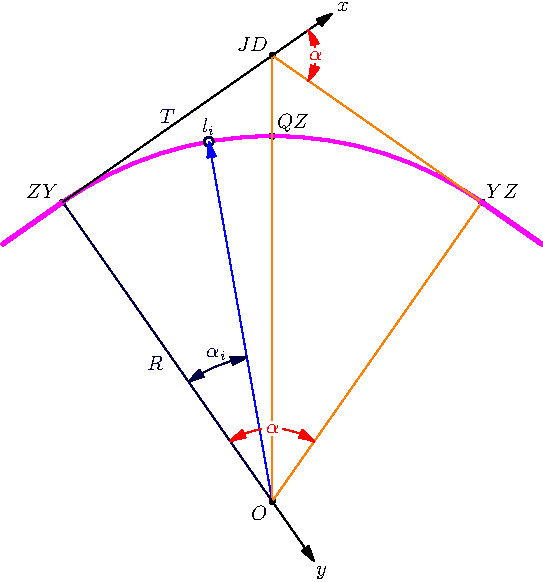
\includegraphics[scale=0.7]{chapter/route/RightCircleRoute.pdf}
    }
    \caption{圆曲线要素图}
    \label{fig:CircleRoute}
\end{figure}


% \begin{figure}[htbp]
%     \centering
%     \includegraphics[scale=0.8]{route/LeftCircleRoute.pdf}
%     \caption{左偏-圆曲线要素图}
%     \label{fig:LeftCircleRoute}
% \end{figure}

% \begin{figure}[htbp]
%     \centering
%     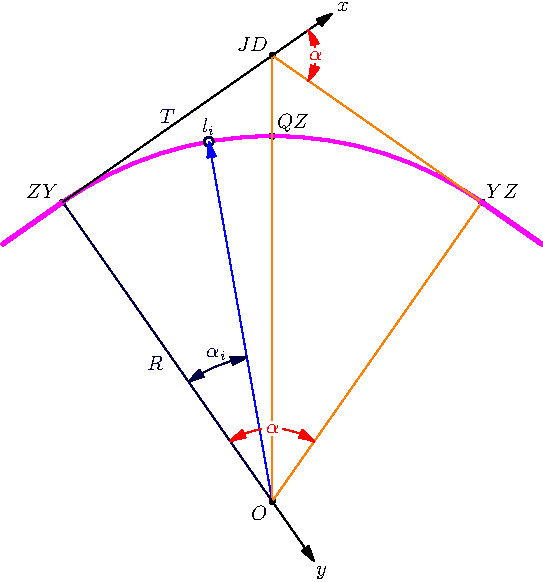
\includegraphics[scale=0.8]{chapter/route/RightCircleRoute.pdf}
%     \caption{右偏-圆曲线要素图}
%     \label{fig:RightCircleRoute}
% \end{figure}

圆曲线的各个要素计算算法如下:

 切线长:$T = R \cdot \tan (\alpha / 2)$

 曲线长:$L = R \cdot \alpha$

 外矢距:$E=R \cdot (\sec (\alpha /2) - 1)$

 切曲差:$q = 2T - L$

 \subsection{圆曲线上点的坐标计算算法分析}

 全站仪的坐标放样模式与 GPS RTK 可以十分方便的进行圆曲线上点的坐标放样。

 尽管圆曲线的计算方法有很多,也比较简单,但为了与后边的缓和曲线计算方法相一致,
 我们在此采用圆心角加半径再加坐标系转换法进行圆曲线上点的坐标计算。

 如图\ref{fig:CircleRoute}所示,以ZY点为原点,以ZY至JD切线方向为x轴,
 以ZY至O点方向为y轴建立ZY切线测量坐标系。从(a)与(b)两图可以看出
无论圆曲线是左偏还是右偏的,其坐标系是一致的。
 在ZY切线坐标系中用极坐标法按如下公式可以计算出圆曲线上任意一点$l_i$的坐标。

圆曲线偏左:

\begin{equation}
\left .
\begin{aligned}
x_{i} &= R \sin \alpha_i   \\
y_{i} &= -R(1- \cos \alpha_i)
\end{aligned}
\right \}
\label{eq:ZYLeftXY}
\end{equation}

圆曲线偏右:

\begin{equation}
\left .
\begin{aligned}
x_{i} &= R \sin \alpha_i   \\
y_{i} &= R(1- \cos \alpha_i)
\end{aligned}
\right \}
\label{eq:ZYRightXY}
\end{equation}

式中:$\alpha_i = l_i / R,  \alpha_i \le \alpha $, $l_i$可用圆曲线上任意一点的里程桩号
减去ZY点的里程桩号。

如果我们以偏右为正、偏左为负,则可以将以上两公式统一,将偏左的Y坐标
乘以 -1 即可。

已知JD的坐标与里程桩号,根据圆曲线的结合几何要素$R, \alpha$即可计算出圆曲线上特征点的
里程桩号:

$KNo_{ZY} = KNo_{JD} - T$

$KNo_{QZ} = KNo_{ZY} + T/2$

$KNo_{YZ} = KNo_{QZ} + T/2$

在ZY切线坐标系中计算出圆曲线上各点的坐标之后,还需将其转换为测量坐标系
(或更正式的称为大地坐标系或独立施工坐标系)。在前一章我们已经做过坐标系的
转换了,在这个线路转换中,我们将ZY-JD边定义为x轴,因此两坐标系的夹角
即为ZY-JD边的坐标方位角,其转换关系如图\ref{fig:xytoxyroute}所示:

\begin{figure}[htbp]
    \centering
    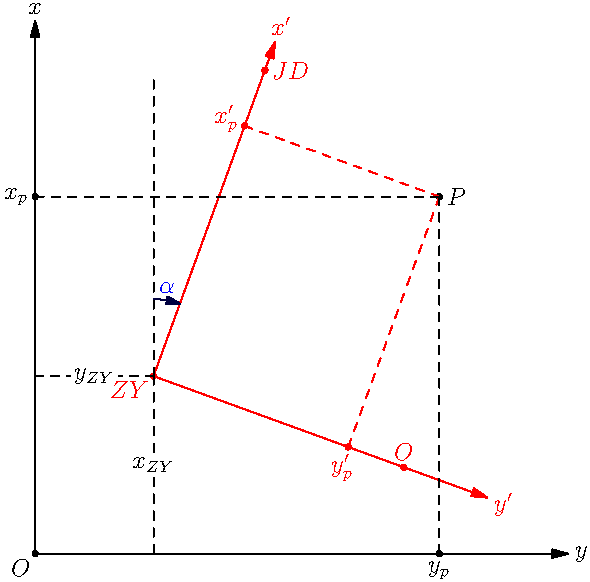
\includegraphics[scale=0.8]{chapter/route/xytoxyroute.pdf}
    \caption{ZY坐标系转测量坐标系}
    \label{fig:xytoxyroute}
\end{figure}

转换公式如下:

\begin{equation}
\left .
\begin{aligned}
x_{P} &= x_{ZY} + x'_P \cos \alpha - y'_P \sin \alpha  \\
y_{P} &= y_{ZY} + x'_P \sin \alpha + y'_P \cos \alpha
\end{aligned}
\right \}
\label{eq:routexytoxy}
\end{equation}


\subsection{圆曲线坐标计算中的类设计}

由以上分析可知,线路计算中至少应该有点类 GPoint 和 线路类 CircleRoute 。

\begin{enumerate}
\item 程序中的点类GPoint

线路上的GPoint 类应包含序号、里程桩号、X坐标、Y坐标、备注信息等内容。
我们设计如下:

\begin{lstlisting}[language=C]
using System;
namespace Route.models
{
    /// <summary>
    /// 点类
    /// </summary>
    public class GPoint : NotificationObject
    {
        private int _no;
        /// <summary>
        /// 序号
        /// </summary>
        public int No
        {
            get { return _no; }
            set
            {
                _no = value;
                RaisePropertyChange("No");
            }
        }

        private double _kno;
        /// <summary>
        /// 里程桩号
        /// </summary>
        public double KNo
        {
            get { return _kno; }
            set
            {
                _kno = value;
                RaisePropertyChange("KNo");
            }
        }

        private double _x;
        /// <summary>
        /// X坐标
        /// </summary>
        public double X
        {
            get { return _x; }
            set
            {
                _x = value;
                RaisePropertyChange("X");
            }
        }

        private double _y;
        /// <summary>
        /// Y坐标
        /// </summary>
        public double Y
        {
            get { return _y; }
            set
            {
                _y = value;
                RaisePropertyChange("Y");
            }
        }

        private string _note;
        /// <summary>
        /// 备注
        /// </summary>
        public string Note
        {
            get { return _note; }
            set
            {
                _note = value;
                RaisePropertyChange("Note");
            }
        }

        public GPoint()
        {
            _no = 0;
            _kno = _x = _y = 0;
            _note = "";
        }
    }
}
\end{lstlisting}

在上面GPoint类中,由于点的里程桩号是double类型,而我们常用的里程桩号是
``K5+200.00''这样的形式,因此我们在类GPoint中设计函数OutKNoInfo()
将其转换输出,其代码如下所示:

\begin{lstlisting}[language=C]
public class GPoint : NotificationObject
{
    //......类中其它代码......

    /// <summary>
    /// 将double类型的kno分解为K5+200.00形式的里程桩号
    /// </summary>
    /// <returns>里程桩号</returns>
    public string OutKNoInfo()
    {
        int k = (int)(_kno / 1000);
        double klength = _kno - k * 1000;
        return string.Format("K{0}+{1:0.000}", k, klength);
    }
}
\end{lstlisting}

以上代码的逻辑非常简单,double类型的里程除以1000,取出公里数,
然后将不足整公里数的部分再取出,然后组合成形如``K5+200.00''这样的
字符串输出。

由于以上代码只涉及类中的 \_kno 字段,因此也可以写成如下的只读属性字段,
调用会更加方便。

\begin{lstlisting}[language=C]
public class GPoint : NotificationObject
{
    //......类中其它代码......

    /// <summary>
    /// 将double类型的kno分解为K5+200.00形式的里程桩号
    /// </summary>
    public string KNoInfo
    {
        get{
            int k = (int)(_kno / 1000);
            double klength = _kno - k * 1000;
            return string.Format("K{0}+{1:0.000}", k, klength);
        }
    }
}
\end{lstlisting}

\item 程序中的圆曲线类CircleRoute

圆曲线类中应包含偏转角$\alpha$、曲率半径R、切线长$T$等基本属性,
还应包括JD点、ZY点、QZ点、YZ点等属性,设计代码如下:

\begin{lstlisting}[language=C]
public class CircleRoute : NotificationObject
{
    private double _alpha;
    /// <summary>
    /// 偏转角,单位:度分秒
    /// </summary>
    public double alpha
    {
        get { return _alpha; }
        set
        {
            _alpha = value;
            RaisePropertyChange("alpha");
        }
    }

    protected double _R;
    /// <summary>
    /// 圆曲线半径
    /// </summary>
    public double R
    {
        get { return _R; }
        set
        {
            _R = value;
            RaisePropertyChange("R");
        }
    }

    double _T;
    /// <summary>
    /// 切线长
    /// </summary>
    public double T
    {
        get { return _T; }
        set
        {
            _T = value;
            RaisePropertyChange("T");
        }
    }

    double _L;
    /// <summary>
    /// 曲线长
    /// </summary>
    public double L
    {
        get { return _L; }
        set
        {
            _L = value;
            RaisePropertyChange("L");
        }
    }

    double _E;
    /// <summary>
    /// 外矢距
    /// </summary>
    public double E
    {
        get { return _E; }
        set
        {
            _E = value;
            RaisePropertyChange("E");
        }
    }

    double _q;
    /// <summary>
    /// 切曲差
    /// </summary>
    public double q
    {
        get { return _q; }
        set
        {
            _q = value;
            RaisePropertyChange("q");
        }
    }

    GPoint _JD = new GPoint();
    /// <summary>
    /// 交点
    /// </summary>
    public GPoint JD
    {
        get { return _JD; }
        set
        {
            _JD = value;
            RaisePropertyChange("JD");
        }
    }

    GPoint _QZ = new GPoint();
    /// <summary>
    /// 曲中点
    /// </summary>
    public GPoint QZ
    {
        get { return _QZ; }
        set
        {
            _QZ = value;
            RaisePropertyChange("QZ");
        }
    }

    GPoint _ZY = new GPoint();
    /// <summary>
    /// 直圆点
    /// </summary>
    public GPoint ZY
	{
		get { return _ZY; }
		set
		{
			_ZY = value;
			RaisePropertyChange("ZY");
		}
	}

    GPoint _YZ = new GPoint();
    /// <summary>
    /// 圆直点
    /// </summary>
    public GPoint YZ
	{
		get { return _YZ; }
		set
		{
			_YZ = value;
			RaisePropertyChange("YZ");
		}
    }

    private int _isLeftRight = 1;
    /// <summary>
    /// 左偏:-1 或 右偏:1
    /// </summary>
    public int IsLeftRight
	{
		get { return _isLeftRight; }
		set
			{
				_isLeftRight = value;
				RaisePropertyChange("IsLeftRight");
			}
    }

    /// <summary>
    /// 线路点集
    /// </summary>
    protected ObservableCollection<GPoint> _pointList =
        new ObservableCollection<GPoint>();

    /// <summary>
    /// 线路点集
    /// </summary>
    public ObservableCollection<GPoint> PointList
    {
        get { return _pointList; }
    }
}
\end{lstlisting}

在圆曲线计算时,由于左偏与右偏的计算是不完全相同的,在此设计一
属性IsLeftRight用来标记。

为了存储计算后的点坐标,我们设计了一点集属性PointList。
\end{enumerate}

\subsection{ 任意桩号点的坐标计算 }

给定任意一桩号,计算圆曲线上点的坐标,函数设计如下:
\begin{lstlisting}[language=C]
/// <summary>
/// 计算任意里程桩号的点坐标
/// </summary>
/// <param name="kno">里程桩号</param>
public void CalSinglePoint(double kno)
{
    double radAlpha = ZXY.SMath.DMS2RAD(alpha);
    T = R * Math.Tan(radAlpha * 0.5);
    L = R * radAlpha;
    E = R * (1 / Math.Cos(radAlpha * 0.5) - 1);

    ZY.KNo = JD.KNo - T;
    QZ.KNo = ZY.KNo + L/2;
    YZ.KNo = QZ.KNo + L/2;

    double li = kno - ZY.KNo;
    if( li<0 || li>L) return; //不是圆曲线上有效范围
    double alphai = li / R;

    GPoint pt = new GPoint();
    pt.KNo = kno;

    pt.X = R * Math.Sin(alphai);
    pt.Y = IsLeftRight * R * (1 - Math.Cos(alphai));

    double A = ZXY.SMath.Azimuth(ZY.X, ZY.Y, JD.X, JD.Y);
    pt.TransformXY(ZY.X, ZY.Y, A); //转换到大地坐标

    PointList.Add(pt); //将计算结果存入PointList
}
\end{lstlisting}

在该算法中,第7行将度分秒形式的偏转角转换为弧度,再根据
前边的算法计算圆曲线的几何要素T、L、E等。

一般情况下JD的里程桩号与坐标是已知的,直圆点ZY的坐标也会已知,但里程桩号
未知,所以需要首先计算出ZY点的里程桩号。同样的道理也可以计算出曲中点QZ与圆
直点YZ点的里程桩号。

第16行根据给定的里程桩号与ZY点的里程桩号计算圆曲线的弧长$l_i$,
第17行做有效性判断:$0 \le l_i \le L$),
第18行根据弧长计算该点所在位置的圆心角$\alpha_i$。

第23、24行根据公式 \ref{eq:ZYRightXY} 计算圆曲线上各点在ZY坐标系
中的各点坐标。如果圆曲线偏左,根据公式 \ref{eq:ZYLeftXY} 将其Y坐标乘以
 -1 即IsLeftRight的属性值即可。

第26行计算出ZY点至JD点的坐标方位角,第27行根据公式\ref{eq:routexytoxy}将其
转换到大地坐标系。

第29行将其加入到PointList列表中,用于界面显示。

\subsection{圆曲线算例与测试代码}
圆曲线的曲率半径为$R=120m$,偏转角为$\alpha=40^{\degree}20'$, 交点JD
的里程桩号为``K3+135.12'',坐标为$(6848.320, 5634.240)$;
直圆点ZY的坐标为$(6821.354,5599.381)$。计算出的圆曲线上各点坐标
如表\ref{tab:YRoute}所示。

\begin{table}[htbp]
\centering
\caption{圆曲线计算示例数据表}
\label{tab:YRoute}
\begin{tabular}{clccl}
\hline
序号  &  里程     &     X    &   Y	  & 备注 \\
\hline
1    & K3+091.05 &  6821.35 & 5999.38 &  ZY \\
2    & K3+100	 & 	6826.56 & 5606.66 &     \\
3    & K3+120	 &  6836.15 & 5624.18 &     \\
4    & K3+133.29 &  6840.85 & 5636.60 &  QZ \\
5    & K3+140	 & 	6842.69 & 5643.06 &     \\
6    & K3+160	 &  6846.02 & 5662.76 &     \\
7    & K3+175.52 &  6846.31 & 5678.27 &  YZ \\
\hline
\end{tabular}
\end{table}

测试代码为:
\begin{lstlisting}[language=C]
models.CircleRoute route = new models.CircleRoute();
route.R = 120;
route.alpha = 40.20;
route.IsLeftRight = 1;

route.JD.X = 6848.320;
route.JD.Y = 5634.240;
route.JD.KNo = 3135.12;

route.ZY.X = 6821.354;
route.ZY.Y = 5599.381;

route.CalSinglePoint(3175.52);
\end{lstlisting}

\subsection{线路上的点按间距批量计算}

除了能进行任意里程桩号的计算外,线路计算程序还应该支持按指定间隔进行
批量计算的功能。在批量计算中,还应该将线路特征点的坐标计算并显示出来,
并按照里程桩号的顺序进行排列。


\subsection{界面的实现}

程序的界面编写我们仍采用WPF技术,布局如图...所示:


\section{有缓和曲线的圆曲线}

有缓和曲线的圆曲线的数学模型与算法相对于圆曲线来说就复杂多了。
下面我们将从算法到程序实现逐一分析。

\subsection{缓和曲线的数学模型}

 \begin{figure}[htbp]
    \centering
    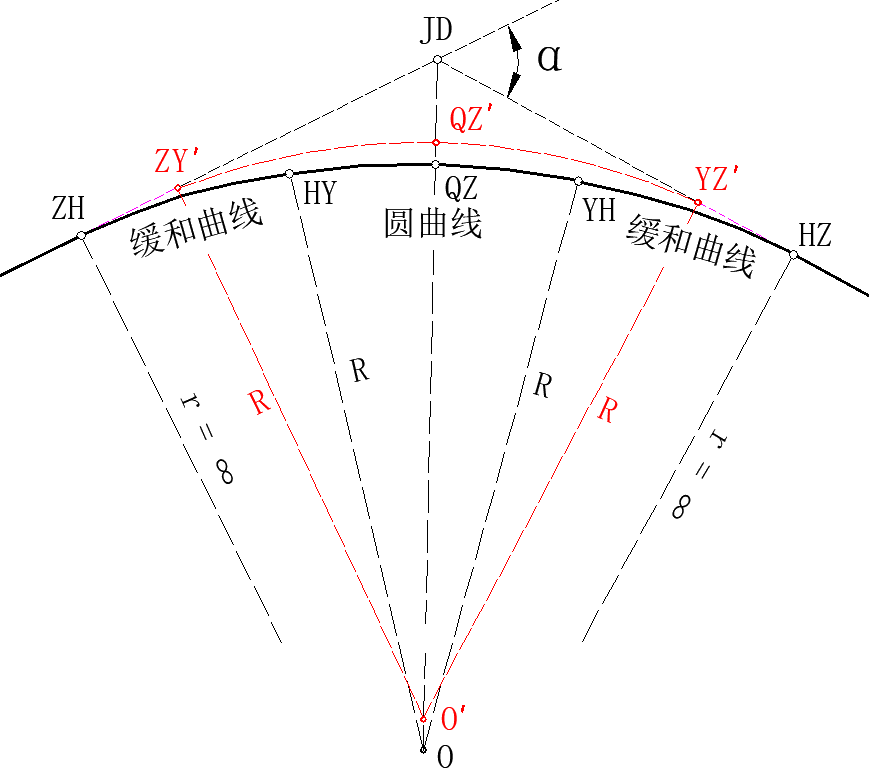
\includegraphics[scale=0.6]{chapter/route/HY01.png}
    \caption{缓和曲线的定义}
    \label{fig:HR01}
\end{figure}


\begin{figure}[htbp]
    \centering
    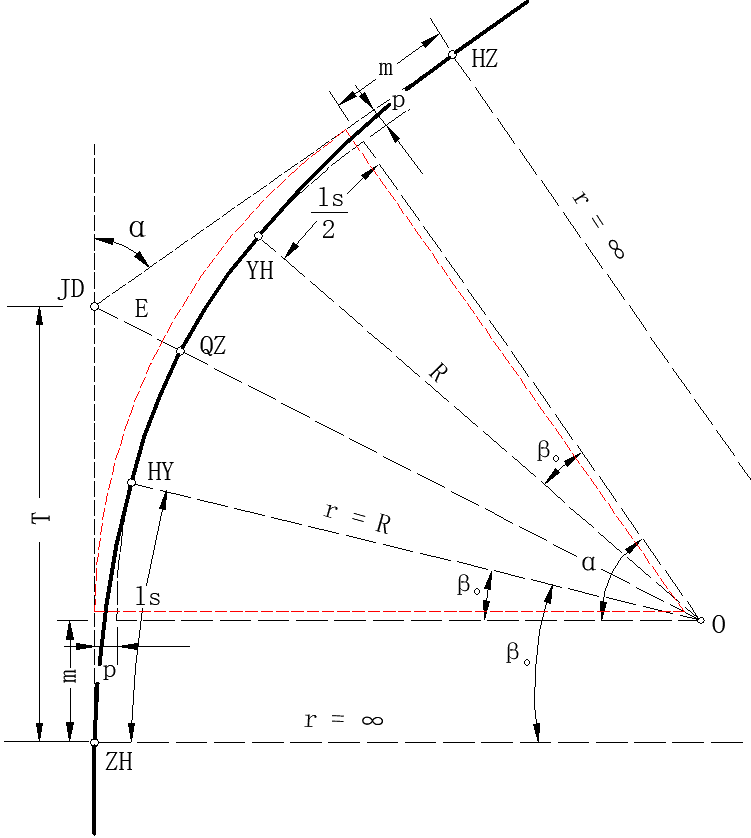
\includegraphics[scale=0.6]{chapter/route/HY02.png}
    \caption{缓和曲线的内移距和切线增长}
    \label{fig:HY02}
\end{figure}


\begin{figure}[htbp]
    \centering
    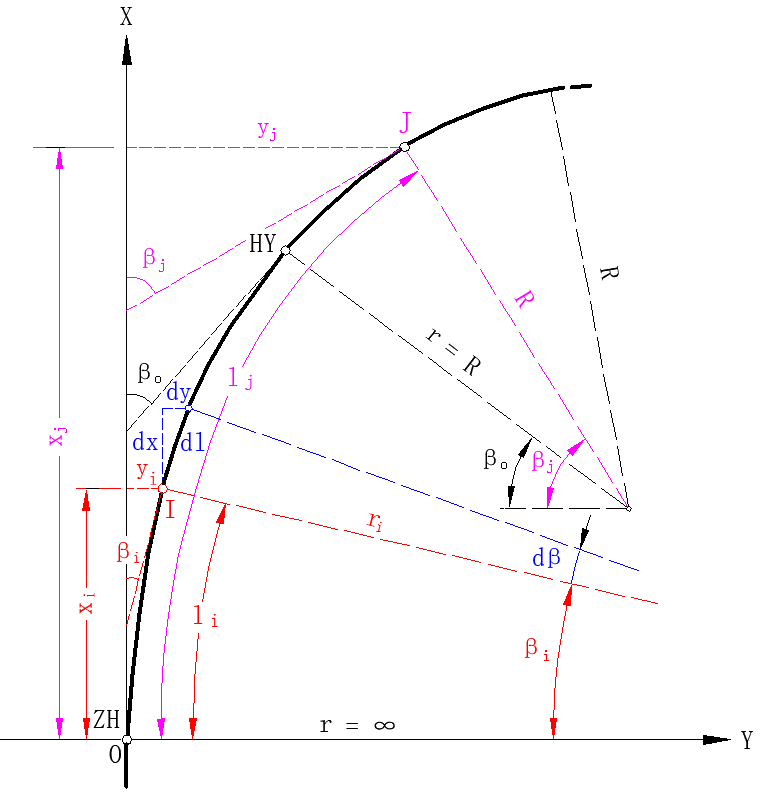
\includegraphics[scale=0.6]{chapter/route/HY03.png}
    \caption{缓和曲线的坐标计算}
    \label{fig:HR03}
\end{figure}

 缓和曲线参数计算公式为:

 $$\beta_0 = \frac{l_0}{2R} $$
切垂距:
$$m=\frac{l_0}{2} - \frac{l^3_0}{240R^2}$$
内移距:
$$p=\frac{l^2_0}{24R}$$


 切线长:$$T = m+ (R+p) \cdot \tan \frac{\alpha}{2}$$

 曲线全长:$$L = R \cdot (\alpha-2\beta_0)  + 2l_0$$

 圆曲线长:$$L_C = R \cdot (\alpha-2\beta_0)$$

 外矢距:$$E=(R+p) \cdot (\sec \frac{\alpha}{2} - 1)$$

\begin{enumerate}

\item  缓和曲线在ZH切线直角坐标系中的坐标计算(ZH段)

以ZH为坐标系原点,ZH至JD方向为x轴,过ZH点垂直于ZH-JD方向为y轴
建立坐标,如图\ref{fig:HY02}所示。则ZH部分缓和曲线上各点的坐标为:

\begin{equation}
\left .
\begin{aligned}
x_i &= l_i - \frac{l^5_i}{40R^2 l^2_0} + \frac{l^9_i}{3456R^4 l^4_0}
           - \frac{l^{13}_i}{599040R^6l^6_0} + ...  \\
y_i &=  \frac{l^3_i}{6Rl_0} - \frac{l^7_i}{336R^3 l^3_0}
    + \frac{l^{11}_i}{42240R^5l^5_0} -\frac{l^{15}_i}{9676800R^7l^7_0}+ ...
\end{aligned}
\right \}
\label{eq:routeZHXY}
\end{equation}

以上公式在计算中取前两项或前三项即可。

\item  缓圆点(HY)坐标计算公式为:

将$l_i = l_0$代入公式\ref{eq:routeZHXY}中计算可得到下式:
\begin{equation}
\left . \begin{aligned}
x_{HY} &= l_0 - \frac{l^3_0}{40R^2} + \frac{l^5_0}{3456R^4}
          - \frac{l^{7}_0}{599040R^6} + ...  \\
y_{HY} &=  \frac{l^2_0}{6R} - \frac{l^4_0}{336R^3}
          + \frac{l^{6}_i}{42240R^5} -\frac{l^{8}_0}{9676800R^7}+ ...
\end{aligned} \right \}
\label{eq:routeHY}
\end{equation}

\item  圆曲线上点的坐标计算公式为:

\begin{equation}
\left . \begin{aligned}
x_{j} &= R \sin \beta_j + m \\
y_{j} &= R(1- \cos \beta_j) +p
\end{aligned} \right \}
\label{eq:routeYQXY}
\end{equation}

式中:$\beta_i = \beta_0 + (l_i - l_0)/R$

\item  缓和曲线在HZ切线直角坐标系中的坐标计算(HZ段)

\begin{figure}[htbp]
    \centering
    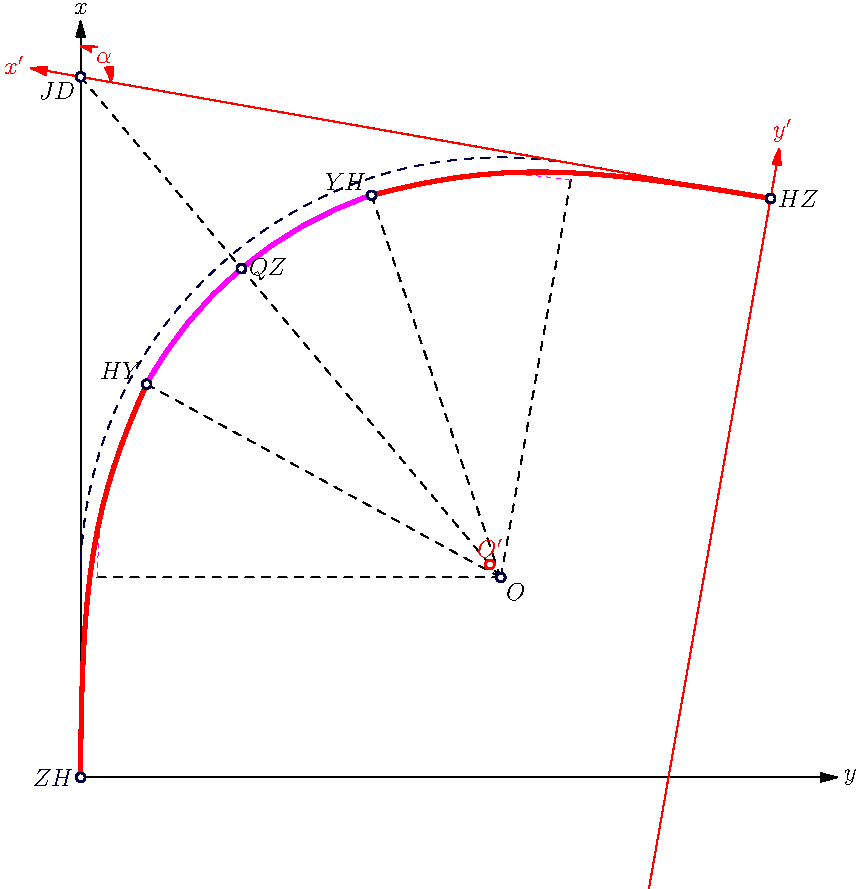
\includegraphics[scale=0.7]{chapter/route/RHY.pdf}
    \caption{缓和曲线的HZ部分坐标计算}
    \label{fig:RHY}
\end{figure}

如图\ref{fig:RHY}所示建立以缓直点HZ为原点,过HZ至JD方向为x轴,
过HZ点的缓和曲线切线为y轴的直角坐标系,计算另一半曲线任意一点的坐标$(x'_i, y'_i)$。
然后,将坐标转换为以ZH点为原点的直角坐标系中。

缓和曲线在HZ坐标系中的坐标可以继续使用公式 \ref{eq:routeZHXY} 计算,然后由图\ref{fig:RHY}
可知将其转换为HZ坐标系中的坐标计算公式为:

\begin{equation}
\left . \begin{aligned}
x'_i &= x_i  \\
y'_i &= - y_i
\end{aligned} \right \}
\label{eq:routeHZPtXY}
\end{equation}

请注意在使用公式 \ref{eq:routeZHXY} 时应将$l_i$替换为 $L-l_i$。

为了将HZ坐标系中的点坐标转换到ZH坐标系中,我们引用公式\ref{eq:routexytoxy}来计算,
请注意公式\ref{eq:routexytoxy}中的$\alpha$为$x'$轴的方位角(即x轴到$x'$轴的水平夹角),
因此图\ref{fig:RHY}应用到公式\ref{eq:routexytoxy}中的$\alpha$ 应为$\alpha + 180 \degree $。
如果将其代入公式\ref{eq:routexytoxy},则有转换公式为:

\begin{equation}
\left . \begin{aligned}
x_i &= x_{HZ} - x'_i  \cos \alpha + y'_i \sin \alpha \\
y_i &= y_{HZ}  -  x'_i \sin \alpha -  y'_i \cos \alpha
\end{aligned} \right \}
\label{eq:routeHZtoZH}
\end{equation}

公式\ref{eq:routeHZtoZH}中的$(x_{HZ}, y_{HZ})$为HZ点在ZH坐标系中的坐标,其值为:

\begin{equation}
\left .
\begin{aligned}
x_{HZ} &= T (1 +  \cos \alpha) \\
y_{HZ} &=  T \sin \alpha
\end{aligned}
\right \}
\label{eq:routeHZXY}
\end{equation}

也可以不用公式\ref{eq:routeHZtoZH},直接将$\alpha+180\degree$代入到
公式\ref{eq:routexytoxy}中进行计算。

在以上计算中,我们以曲线右偏为例的,如果曲线左偏,同样的方法建立坐标系,
x坐标是相同的, y坐标乘以 -1 即可。

\item 曲线上点坐标转换为大地坐标的计算公式为:

由于已经将曲线上的点坐标统一到ZH坐标系中了,我们继续引用公式\ref{eq:routexytoxy}
将ZH切线坐标系坐标转换到大地坐标系(测量坐标系)中,公式中的$\alpha$为$ZH \rightarrow JD$
的坐标方位角。

\end{enumerate}


\subsection{有缓和曲线的圆曲线算例}

缓和曲线的曲率半径$R=1000$,偏转角$\alpha =10.1820$, 右偏,
缓和曲线长$l_0=80$,直缓点ZH的坐标为$(3088256.238, 66798.566)$,
交点JD的坐标为$(3088386.436, 66798.566)$,里程桩号为``K5+5330.198''。
计算出的曲线上各点坐标如表\ref{tab:HYRoute}所示。

\begin{table}[htbp]
\centering
\caption{有缓和曲线的圆曲线计算示例数据表}
\label{tab:HYRoute}
\begin{tabular}{ccccl}
\hline
序号 & 里程	    &        X	   &      Y	   &  备注 \\
\hline
1   & K5+200.000 & 3088256.238 & 66798.566 &  ZH  \\
2   & K5+220.000 & 3088276.238 & 66798.583 &      \\
3   & K5+240.000 & 3088296.238 & 66798.699 &      \\
4   & K5+260.000 & 3088316.235 & 66799.016 &      \\
5   & K5+280.000 & 3088336.225 & 66799.632 &  HY  \\
6   & K5+300.000 & 3088356.200 & 66800.632 &      \\
7   & K5+320.000 & 3088376.150 & 66802.031 &      \\
8   & K5+329.933 & 3088386.048 & 66802.874 &  QZ  \\
9   & K5+339.866 & 3088395.936 & 66803.815 &      \\
10  & K5+359.866 & 3088415.815 & 66806.008 &      \\
11  & K5+379.866 & 3088435.646 & 66808.598 &  YH  \\
12  & K5+399.866 & 3088455.424 & 66811.568 &      \\
13  & K5+419.866 & 3088475.156 & 66814.834 &      \\
14  & K5+439.866 & 3088494.853 & 66818.297 &      \\
15  & K5+459.866 & 3088514.534 & 66821.858 &  HZ  \\
\hline
\end{tabular}

\end{table}

\section{较为完整的线路里程桩计算}

以上曲线要素的计算是按曲线类型单独进行分析编写的,实际上一条线路
是由无数段直线、圆曲线与缓和曲线组成。


